%%
%% 研究報告用スイッチ
%% [techrep]
%%
%% 欧文表記無しのスイッチ(etitle,eabstractは任意)
%% [noauthor]
%%

%\documentclass[submit,techrep]{ipsj}
\documentclass[submit,techrep,noauthor]{ipsj}

\usepackage[dvips]{graphicx}
\usepackage{latexsym}

%画像用の追加
%\usepackage[dvipdfmx]{graphicx}

\def\Underline{\setbox0\hbox\bgroup\let\\\endUnderline}
\def\endUnderline{\vphantom{y}\egroup\smash{\underline{\box0}}\\}
\def\|{\verb|}
%

%\setcounter{巻数}{59}%vol59=2018
%\setcounter{号数}{10}
%\setcounter{page}{1}


\begin{document}

\title{Tableau CRMのEinstein Discovery ストーリーによる\\株価指標に着目した日経平均株価分析の試み}

\etitle{An Attempt to Analysis of Nikkei Stock Average Focused on \\A Stock indexes Using Einstein Discovery Story of Tableau CRM}

\affiliate{LA}{ロジカル・アーツ株式会社\\
Logical Arts Corporation, Osaka, Osaka 541--0054, Japan}

\author{輪島 幸治}{Koji Wajima}{LA}[wajima@logical.co.jp,kwajima@ce.slis.tsukuba.ac.jp,wajimak@nict.go.jp]

\begin{abstract}
%現状分析
近年,スマートフォンによるオンライントレードや,
少額投資非課税制度(NISA)などの非課税口座の登場で,株式の取引が盛んに行われている.
日本の株式市場における相場の動向を測る代表的な株価指数に,日経平均株価指数がある.
%これまで,日経平均株価指数は多くの各国の株価指数との比較分析が行われてきた.
%
%解決策提示
本研究では,日経平均株価指数を目標変数,説明変数を各国における代表的な株価指数で,
一般化線形モデル(GLM:Generalized Linear Model)を用いてモデルを構築する.
GLMで作成したモデルを用いて精度,各株価指標との相関性,予測値と実績値を算出して,
日経平均株価指数と各国の主要株価指数値について考察する.
%
%提案手法の特徴
本研究の特徴は,各国における代表的な株価指数をモデル作成のデータに用いていることから,
各国における経済動向や連動性を包含した分析が期待できる.
また,モデル作成をして評価していることから,他の株価指数との単純な相関性だけでなく,
予測精度や誤差などの10種類以上の網羅的な評価指標で評価している.
本研究では提案手法の実装を網羅的かつ一意的な分析が期待できるクラウドAI分析プラットフォームであるTableau CRMで実装した.

%分かったこと
目標変数を日経平均株価指数,説明変数を他国の主要な株価指数を用いて作成した一般化線形モデルで,
有効な決定係数値が得られた.また,相関性が高い株価指数を明らかにした.
加えて,Tableau CRMのEinstein Discovery ストーリーを用いて日経平均株価が最高になるケース,
最低になるケース,平均よりも優れていたケース,
悪かったケースにおける他国の主要な株価指数を考察した.結果を報告する.

\end{abstract}


%
%\begin{jkeyword}
%情報処理学会論文誌ジャーナル,\LaTeX,スタイルファイル,べからず集
%\end{jkeyword}
%
%\begin{eabstract}
%This document is a guide to prepare a draft for submitting to IPSJ
%Journal, and the final camera-ready manuscript of a paper to appear in
%IPSJ Journal, using {\LaTeX} and special style files.  Since this
%document itself is produced with the style files, it will help you to
%refer its source file which is distributed with the style files.
%\end{eabstract}
%
%\begin{ekeyword}
%IPSJ Journal, \LaTeX, style files, ``Dos and Dont's'' list
%\end{ekeyword}

\maketitle

%1
\section{はじめに}
%現状分析
近年,スマートフォンによるオンライントレードや
少額投資非課税制度(NISA)などの非課税口座の登場で,
株式の取引が盛んに行われている.
%
株式の相場においては,市場の状況を示すために,
株価や株価の変動を表示する株価指数と呼ばれる指標が用いられている.
%
代表的な日本の指標には,東京証券取引所に一部上場する主要225銘柄から算出された日経平均株価指数と呼ばれる株価指数がある.
%日経平均株価指数は,東京証券取引所に一部上場する主要225銘柄から算出された株価指標であり,
日経平均株価指数は,東京証券取引所の相場動向を測る指標として用いられている.
これまで,日経平均株価指数は多くの各国の株価指数との比較分析が行われてきた.

\newpage
%課題提示
昨今,新型コロナウイルスに端を発した在宅勤務の増加により,
クラウドアプリケーションやオンラインミーティングアプリケーションなど,
飛躍的に伸びている海外製のWebサービスも多く見られるようになってきた.
%
そこで本研究では,海外株価指標を用いて,
日経平均株価を予測して分析することを試みた.

%解決策
本研究では,日経平均株価指数に対する各国の主要な株価指数を用いて分析を行う.
各国の主要な株価指数で日経平均株価指数を分析することで,
相関性や日経平均株価指数が高い場合における他の株価指数を明らかにすることが期待できる.


%提案手法の特徴
本研究における提案では,日経平均株価指数を目標変数,
9種類の各国主要株価指数を説明変数として設定して作成した
一般化線形モデル(GLM:Generalized Linear Model)で分析を試みる.
%
日経平均株価指数を目標値に設定してGLMで予測を行う.
また,日経平均株価指数が大きくなった場合における各国主要株価指数の値についても考察する.

\newpage
本研究では,別の指標値との相関性分析だけではなく,
GLM分析で目標値に対する予測精度や誤差についても考察した.
加えて,本研究の特徴は,目標変数が優れた値を取った際の
各国の主要株価指数が取る値についても考察した.

%評価結果
提案手法の有効性は,R$^2$や平均絶対誤差 (MAE) など
10種類の網羅的な評価指標を4分割交差検証で評価した.
結果,R$^2$において,有効性が得られた.
また,目標変数に対する各種誤差や各国主要株価指数における状況を明らかにして,
他国の株価指数が与える影響についても明らかにした.
%
加えて,提案手法の実装をクラウドAI分析プラットフォームである
Tableau CRMを用いて行うことで,迅速かつ一意的な分析を行った.
結果を報告する.

%論文の構成
本論文では,2章で関連研究に関して述べる.
3章で本研究で用いる一般化線形モデルについて詳述する.
4章では,提案手法の評価実験内容について述べ,
5章で実験結果を示す.最後にまとめと今後の課題を示す.

%2
\section{関連研究}
日経平均株価指数を分析する研究には,イベントから考察する研究,
外部の情報で分析する研究,アルゴリズムに基づく研究などがある.
%
イベントから考察した研究には,米国同時多発テロ直後に225銘柄中,
120銘柄がストップ安となった大規模マクロショック発生時を論じる研究\cite{gendaifinance01}.
日経平均株価指数を構成する構成銘柄30銘柄入れ替え時を論じる研究\cite{gendaifinance02}などがある.
%
外部の情報を用いる研究には,金融経済日報をテキストマイニングしたデータで
市場変動の要因分析を行う研究\cite{financialmarkets01}\cite{financialmarkets02}などがある.
%
アルゴリズムに基づく研究には,ベイジアンネットワークを用いた株価予測を行う研究\cite{weko79192}などがある.
%
加えて,株価指数を対象とした研究には,金融ニュースを用いる研究\cite{financialnewsarticles}など多くの研究が行われている.

本研究は,GLMを用いて,日経平均株価指数を各国の主要株価指数を用いて株価指標の予測を行う.
このため,外部の情報とアルゴリズムに基づいて株価指数を予測する研究である.
%
なお,本研究は\ref{experiment}節にて後述するが,分析対象期間が2000年1月から2022年1月までと長い.
したがって,米国同時多発テロやリーマンショックのような大規模マクロショックが発生時期についてもも含めて評価している.

さて,データ分析では,起こった出来事や事実から必要なものを選別・分析を行い,
価値観を加えることで,新たな知見が得られるとされている\cite{nttdata}.
一方で,新たな課題に対して,分析を行う場合,実装のコストや妥当性,
評価指標の網羅性における課題が存在する.
%
このため,本研究では,入力に対して,網羅的かつ一意的な結果が得られ,
かつGUIの画面操作にて分析結果が得られる
クラウドAI分析プラットフォームの一つであるTableau CRMを用いた.

\newpage
\section{概要}
\vspace{-2mm}
本節では,日経平均株価指数を予測する際に用いるアルゴリズムのGLMについて概説する.
加えて,GLMモデル作成や相関性分析で説明変数となる各国の主要株価指数についても概説する.

%3.1
\vspace{-2mm}
\subsection{一般化線形モデル}
本研究で用いる一般化線形モデル(GLM:Generalized Linear Model)について概説する.
まず,目的変数を$ Y_{1},Y_{2},...Y_{n}$とした一般線形モデルを式(\ref{generalliner})に示す.

\begin{equation}
\label{generalliner}
Y=X \beta + \varepsilon 
\end{equation}

式(\ref{generalliner})のとき,目的変数Yは$Y=(Y_{1},Y_{2},...Y_{n})^{T}$と置く.Xは$n \times K$行列のデータ行列を表す.
また,$ \beta $は係数パラメータであり,$\beta=( \beta_{1}, \beta_{2},... \beta_{k})^{T}$と置き,
$\varepsilon$は,独立に$N(0, \sigma^{2})$に従う確率変数を表す.
%
この時,$Y_{i}$が指数分布族に属する分布に従うものとして,単調で微分可能な関数$g(x)$を用いることで,
GLMモデルを表すことができる.GLMモデルを式(\ref{GLM})に表す.

\begin{equation}
\label{GLM}
g(E[Y])=X \beta 
\end{equation}

式(\ref{GLM})のとき,$g(x)$を連結関数と呼び,$X \beta $は線形予測子と呼ばれる.
ここで,$g(E[Y])$は,$(g(E[Y_{1}]),...,g(E [Y_{n}]))^{T}$である.
本研究では,目的変数Yに日経平均株価の値,データ行列に各国の主要株価指数を用いている.
このため,各国の主要株価指数から連結関数$g(x)$をモデル化して,予測することで,評価した.

%3.2
\subsection{本研究で用いる各国の株価指数}
本研究で用いる各国の株価指数を表\ref{tab:tickersymbol}に示す.
本研究で選定した各国の株価指数は,日本経済新聞社が提供している"nikkei4946.com"の
経済ナレッジバンクにある経済用語に記載している世界の主要株価指数から,
Google Financeで取得可能な株価指数を用いている.

\begin{table}[h] 
\caption{各国における主要な株価指数} 
%\ecaption{An Example of Table.}
\label{tab:tickersymbol}
\hbox to\hsize{\hfil
\begin{tabular}{l|l}\hline\hline
ティッカーシンボル & 評価指標値 \\\hline \hline
\scriptsize{INDEXNIKKEI:NI225} & 日経平均株価 \\\hline
\scriptsize{INDEXTOPIX:TOPIX} & 東証株価指数 \\\hline
\scriptsize{INDEXDJX:.DJI} & ダウ平均株価 \\\hline
\scriptsize{INDEXSP:.INX} & S\&P 500種株価指数(S\&P 500) \\\hline
\scriptsize{INDEXHANGSENG:HSI} & 香港ハンセン指数 \\\hline
\scriptsize{INDEXBOM:SENSEX} & SENSEX指数 \\\hline
\scriptsize{INDEXFTSE:UKX} & FTSE100種総合株価指数 \\\hline
\scriptsize{INDEXDB:DAX} & ドイツ株式指数 \\\hline
\end{tabular}\hfil}
\end{table}

表\ref{tab:tickersymbol}の8種類の株価指数のうち,
本研究では"INDEXNIKKEI:NI225"の値を目的変数,
"INDEXNIKKEI:NI225"以外の株価指数をGLMでモデル作成に使用するデータとして用いる.

\newpage
%4
\section{実装}

%4.1
\subsection{実験環境}\label{experiment}
%値取得
本研究では,Google サービスの一つであるGoogle Finance\footnote{Google Finance:https://www.google.com/finance/}のデータをGoogle WorkspaceのGoogle スプレッドシート\footnote{Google Workspace:https://workspace.google.co.jp/}を用いて取得している.
Google スプレッドシートでは,`GOOGLEFINANCE`関数を使用することで,
証券のティッカーシンボル、開始日、終了日を指定して現在、過去の証券情報を取得することができる.

本研究では,`GOOGLEFINANCE`関数で取得した証券情報の値をCSVファイル化して使用している.
%2021年9月19日現在のGoogle Financeのデータは,
%Morningstar社,Thomson Reuters社,ICE Data Servicesから提供されている.
%
取得期間は評価に用いる日経平均株価が取得できる最も古い日時である1991年1月25日から,
2022年1月28日までの11,326日間(約31年分)のGoogle Finance上のデータをGoogle スプレッドシートで指定して取得した.
%
評価実験では,日経平均株価だけでなく,各国における株価指標を用いる.
このため取得可能期間の都合上,2000年1月5日から2022年1月28日までの8,059日間(約22年分)のデータから,
月曜日から金曜日までの平日のみを対象に評価対象データを作成している.
なお,値が取得できなかった日については,0で値を補完している.

ここで,本研究では,提案手法の実装をTableau CRMのEinstein Discoveryにて行っている.
分析に使用しているTableau CRMだが,Salesforceで有効化して使用する機能の一つであり,
Salesforce上で動作するAI分析プラットフォームであることから,
Tableau CRMが有効なDeveloper Edition組織を作成して検証を行った\footnote{\scriptsize{https://trailhead.salesforce.com/en/promo/orgs/analytics-de}}.

%4.2
\subsection{本研究で用いるモデルの評価方法}
本研究では,一般化線形モデルの実装および評価をTableau CRMのEinstein Discoveryで行っている.
Tableau CRMにおける評価可能な項目および本研究の評価で用いる評価指標を下記に示す.

\begin{description}
   \item[概要(1)目的変数を予測]\mbox{}\\
            ・決定係数\\
            ・結果変数の分布\\
            ・上位の予測因子
\end{description}
%
\begin{description}
   \item[モデル評価(1)全体的なパフォーマンス]\mbox{}\\
            ・決定係数,MAE,RMSE\\
            ・予測 vs 実際プロット\\
            ・標準化された残差の正規 QQ プロット
   \item[モデル評価(2)4分割交差検証]\mbox{}\\
            ・行の数,$R^{2}$,平均絶対誤差(MSE),二乗平均平方根誤差(RMSE),平均絶対誤差(MAE),二乗平均平方根対数誤差(RMSLE),残差逸脱度(Residual Deviance),\\
             平均残差逸脱度(Mean Residual Deviance),\\Null 逸脱度(Null Deviance),Null 自由度(Null Degrees of Freedom),残差自由度(Residual Degrees of Freedom)
   \item[モデル評価(3)モデル係数]\mbox{}\\
	   ・変数の数,相互関係が含まれる変数の数,切片
\end{description}
%
\begin{description}
   \item[予測検査(1)トレーニングデータセットの検査]\mbox{}\\
            ・予測,実績,残差,パーセント
\end{description}

%4.3
\subsection{Tableau CRMのインサイトによる評価}
Tableau CRMのEinstein Discoveryでは,目的変数の評価をモデルで行う際に,
インサイトと呼ばれる他の指標値との比較を行う機能がある.
インサイトとは,洞察の意だが,Tableau CRMにおけるインサイトは,
説明変数が特定の値だった場合に,目的変数の値が平均よりも良い場合など
目的変数に対する説明変数の状態を分析する機能である.
%
算出された本研究では,説明変数の状態をもとに考察を行う.
Tableau CRMのインサイト機能における評価例を下記に示す.

\begin{itemize}
\item 目的変数が最高 になるのはいつ?
\item 目的変数が最低 になるのはいつ?
\item 平均よりも優れていたケース
\item 平均よりも悪かったケース
\item 他より優れていたケース
\item 他よりも悪化したケース
\end{itemize}

本研究では,一般化線形モデルの評価に加えて,
インサイト機能を用いて,目的変数である日経平均株価に対する
各国株価指数の影響を評価する.

%5
\section{評価実験}
Tableau CRMで日経平均株価を目的変数として,
GLMアルゴリズムで作成したモデルの評価結果を\ref{evaluation1}節から\ref{evaluation3}節に示す.

\subsection{モデル評価結果 - 概要(1)}\label{evaluation1}
%作成モデルで行った評価結果の概要を図\ref{INDEXNIKKEI_NI225_ReviewModelAccuracy},
%図\ref{INDEXNIKKEI_NI225_TrainingDataandtheModel}および
作成モデルで行った評価結果の概要を図1,図2および
表\ref{tab:INDEXNIKKEI_NI225_correlation}に示す.
%
%図\ref{INDEXNIKKEI_NI225_ReviewModelAccuracy}は,GLMで日経平均株価を予測した際の決定係数のグラフである.
%図\ref{INDEXNIKKEI_NI225_TrainingDataandtheModel}は,日経平均株価の値の頻度分布を示すヒストグラムである.
図1は,GLMで日経平均株価を予測した際の決定係数のグラフである.
図2は,日経平均株価の値の頻度分布を示すヒストグラムである.
表\ref{tab:INDEXNIKKEI_NI225_correlation}は,モデル作成に用いたデータとの相関性を表す表である.

得られた結果から,決定係数が7割以上を超えていることから,一定の精度で予測が行える.
日経平均株価の分布状況については,$9,201-12,268$のレンジで1.5kを示す区間の値が最も分布が多い.
モデル作成に使用したデータでは,東証株価指数との相関性が最も高い結果が得られた.

\newpage
% 図の挿入
\begin{figure}[h]
\begin{center}
\label{INDEXNIKKEI_NI225_ReviewModelAccuracy}
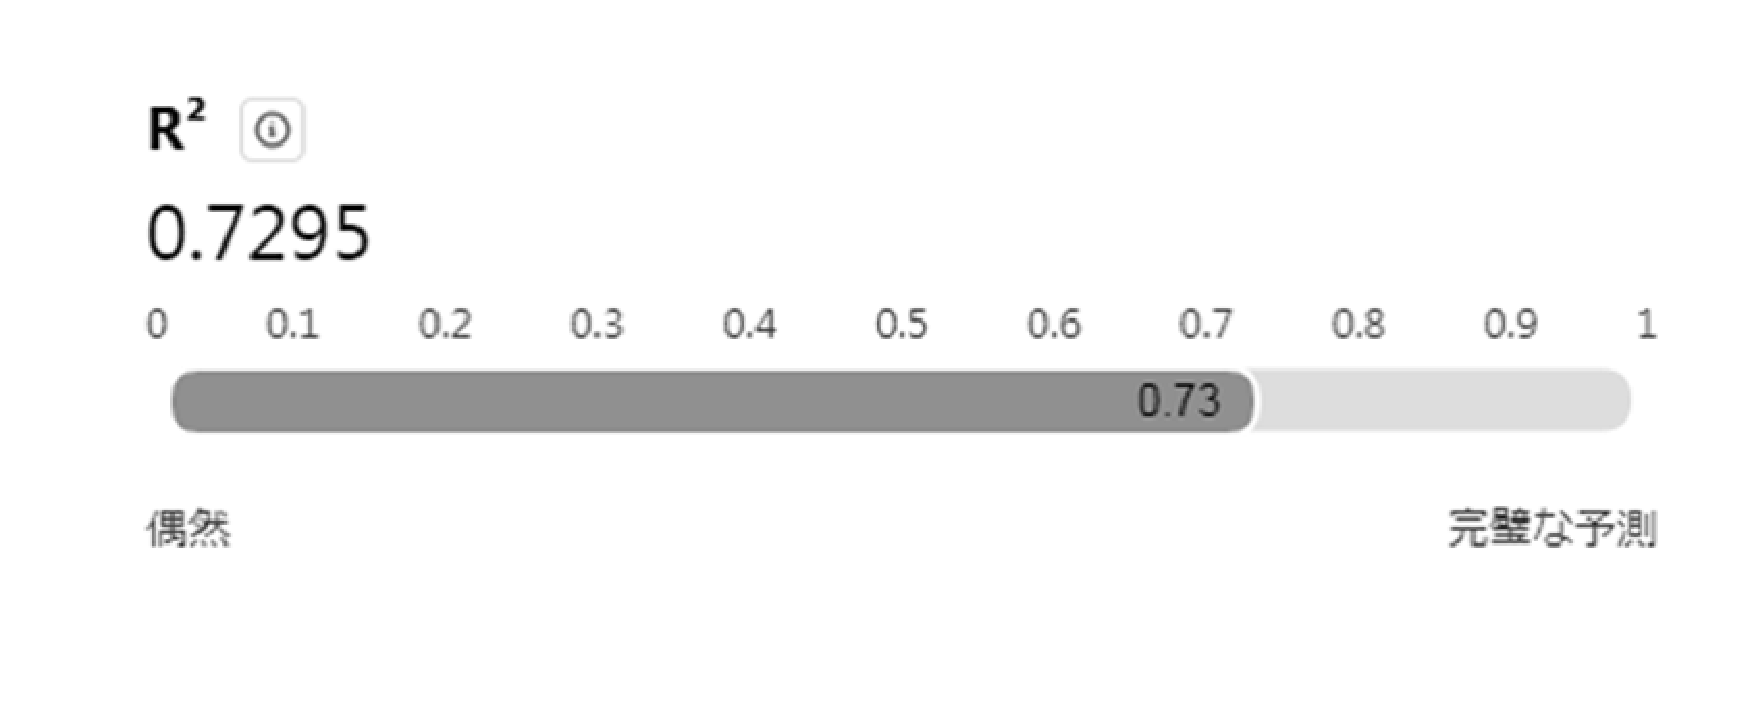
\includegraphics[width=\linewidth]{./eps/INDEXNIKKEI_NI225_ReviewModelAccuracy.eps}
\caption{モデルの精度}
\vspace{-2mm}
\end{center}
\end{figure}
\vspace{-4mm}
% 図の挿入
\begin{figure}[h]
\begin{center}
\label{INDEXNIKKEI_NI225_TrainingDataandtheModel}
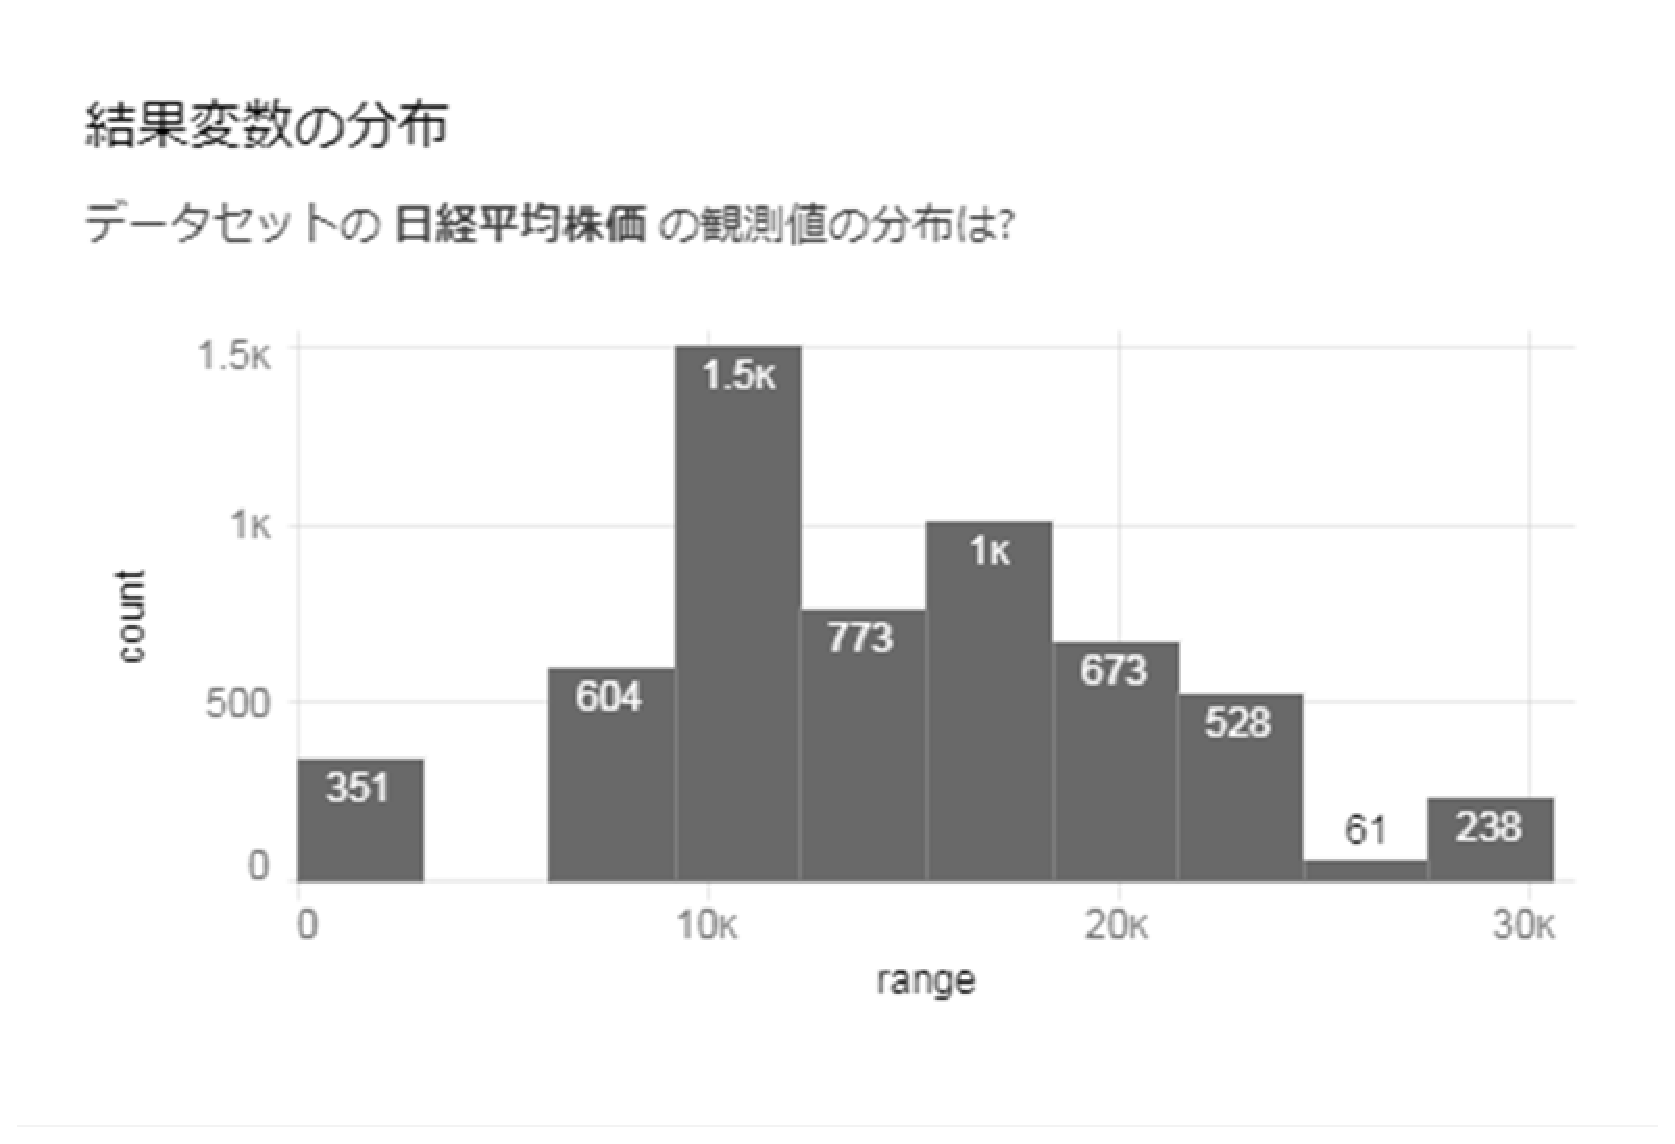
\includegraphics[width=\linewidth]{./eps/INDEXNIKKEI_NI225_TrainingDataandtheModel.eps}
\caption{結果変数の分布}
\vspace{-2mm}
\end{center}
\end{figure}
\vspace{-2mm}
\begin{table}[h] 
\caption{表の例} 
\label{tab:INDEXNIKKEI_NI225_correlation}
\hbox to\hsize{\hfil
\begin{tabular}{c||c|c}\hline\hline
項番 & 変数 & 結果との相関関係\\\hline
1 & 東証株価指数 &81.44\% \\\hline
2 & ドイツ株式指数 &49.96\% \\\hline
3 & S\&P 500種株価指数 &49.44\% \\\hline
4 & ダウ工業株30種平均 &46.57\% \\\hline
5 & SENSEX指数 & 43.14\% \\\hline
6 & FTSE100種総合株価指数 & 41.22\% \\\hline
7 & 香港ハンセン指数 &34.47\% \\\hline
\end{tabular}\hfil}
\newpage
\end{table}
\vspace{-2mm}

%5.1
\subsection{モデル評価(1)全体的なパフォーマンス}\label{evaluation2}
次に,Tableau CRMにて作成したGLMモデルを用いて,
予測値と実測値を比較評価した結果を,
%表\ref{INDEXNIKKEI_NI225_performance},図\ref{INDEXNIKKEI_NI225_PredictedvsActual}および
%図\ref{INDEXNIKKEI_NI225_NormalQQPlot}に示す.
表\ref{INDEXNIKKEI_NI225_performance},図3および図4に示す.

\vspace{-2mm}
\begin{table}[h] 
\caption{全体的なパフォーマンス} 
\label{INDEXNIKKEI_NI225_performance}
\hbox to\hsize{\hfil
\begin{tabular}{c||c|c}\hline\hline
項番 & 指標 & 値\\\hline \hline
1 & $R^{2}$ & 0.7295 \\\hline
2 & MAE & 1720.43 \\\hline
3 & RMSE & 3385.78 \\\hline
\end{tabular}\hfil}
\end{table}

% 図の挿入
\begin{figure}[h]
\begin{center}
%\label{INDEXNIKKEI_NI225_PredictedvsActual}
\label{PredictedvsActual}
\includegraphics[width=\linewidth]{./eps/INDEXNIKKEI_NI225_PredictedvsActual.eps}
\caption{予測 vs 実際}
\end{center}
\end{figure}

% 図の挿入
\begin{figure}[h]
\begin{center}
\label{INDEXNIKKEI_NI225_NormalQQPlot}
\includegraphics[width=\linewidth]{./eps/INDEXNIKKEI_NI225_NormalQQPlot.eps}
\caption{標準化された残差の正規 QQ プロット}
\end{center}
\end{figure}

表\ref{INDEXNIKKEI_NI225_performance}から,
決定係数,予測誤差といった一般的な指標値が得られた.
予測誤差については,値が小さければ良いが,
今回は比較対象となる目標変数がない.このため,得られた値は参考値である.

%図\ref{INDEXNIKKEI_NI225_PredictedvsActual}については,
図3については,
予測結果に対する実際の値がプロットされた図だが,
0で値を補完した一部の値を除けば,予測された値の周辺に実際の値が分布されている.
ゆえに,概ね妥当な予測が得られたことがわかった.

\newpage
%図\ref{INDEXNIKKEI_NI225_NormalQQPlot}については,
図4については,
残差が正規分布であるかを判断する正規性の判断を用いるためのグラフである.
残差とは,目標変数のデータの値と予測値との差である.
評価結果では,正規分布ではなく,非正規分布に近い結果が得られた.

%\begin{table}[tb] 
%\caption{表の例} 
%\ecaption{An Example of Table.}
%\label{tab:example}
%\hbox to\hsize{\hfil
%\begin{tabular}{l|lll}\hline\hline
%& column1 & column2 & column3 \\\hline
%row1 &	item 1,1 & item 2,1 & ---\\
%row2 &	---      & item 2,2 & item 3,2 \\
%row3 &	item 1,3 & item 2,3 & item 3,3 \\
%row4 &	item 1,4 & item 2,4 & item 3,4 \\\hline
%\end{tabular}\hfil}
%\end{table}
%\clearpage

%5.2
\vspace{-2mm}
\subsection{モデル評価(2)4分割交差検証}\label{evaluation3}
作成したモデルを10種類の評価指標で評価した結果を
表\ref{CrossValidation1}から表\ref{CrossValidation4}に示す.
評価に用いた10種類の評価指標は,Tableau CRMの評価指標である
R$^2$,MSE,RMSE,MAE,RMSLE,
Residual Deviance,Mean Residual Deviance,
Null Deviance,Null Degrees of Freedom,Residual Degrees of Freedomの10種類である.
\vspace{-2mm}

\begin{table}[h] 
\caption{GLMモデルの評価(交差検証 - 誤差)} 
\label{CrossValidation1}
\hbox to\hsize{\hfil
\begin{tabular}{c||c|c|c|c}\hline\hline
& Fold 1 & Fold 2 & Fold 3 & Fold 4 \\\hline \hline
R$^2$ & 0.937 & 0.94 & 0.946 & 0.942 \\\hline
MSE & \tiny{2628827.39} & \tiny{2550186.54} & \tiny{2201378.73} & \tiny{2408838.51} \\\hline
RMSE & 1621.37 & 1596.93 & 1483.7 & 1552.04 \\\hline
MAE & 800.67 & 830.8 & 777.31 & 803.66 \\\hline
RMSLE & \footnotesize{undefined} & \footnotesize{undefined} & \footnotesize{undefined} & \footnotesize{undefined} \\\hline
\end{tabular}\hfil}
\end{table}
\vspace{-2mm}

\begin{table}[h]
\caption{GLMモデルの評価(交差検証 - その他)} 
\label{CrossValidation2}
\hbox to\hsize{\hfil
\begin{tabular}{c||c|c}\hline\hline
 & 残差逸脱度 & Mean 平均残差逸脱度 \\\hline \hline
Fold 1 & 3067841564.32 & 2628827.39 \\\hline
Fold 2 & 2764402209.47	 & 2550186.54 \\\hline
Fold 3 & 2540391060.13 & 2201378.73 \\\hline
Fold 4 & 2905059240.56 & 2408838.51 \\\hline
\end{tabular}\hfil}
\end{table}

\begin{table}[h]
\caption{GLMモデルの評価(交差検証 - その他)} 
\label{CrossValidation3}
\hbox to\hsize{\hfil
\begin{tabular}{l||l}\hline\hline
 & Null 逸脱度 \\\hline\hline
Fold 1 & 48665658103.48 \\\hline
Fold 2 & 46072534557.2 \\\hline
Fold 3 & 46991636312.67 \\\hline
Fold 4 & 50631643833.43 \\\hline
\end{tabular}\hfil}
\end{table}

\begin{table}[h] 
\caption{GLMモデルの評価(交差検証 - その他)} 
%\ecaption{An Example of Table.}
\label{CrossValidation4}
\hbox to\hsize{\hfil
\begin{tabular}{c|c|c}\hline\hline
 & \tiny{Null 自由度} & \tiny{残差自由度} \\\hline
Fold 1 & 1166 & 981 \\\hline
Fold 2 & 1083 & 898 \\\hline
Fold 3 & 1153 & 968 \\\hline
Fold 4 & 1205 & 1020 \\\hline
\end{tabular}\hfil}
\end{table}

\newpage
表\ref{CrossValidation1}における決定係数$R^{2}$の結果から,
交差検証を行った場合は,90\%以上の決定係数の値が得られた.
%
節\ref{evaluation2}においても前述したが,
表\ref{CrossValidation1}における予測誤差の評価指標については,
比較対象がないため今回は参考値である.
%
表\ref{CrossValidation4}で得られた自由度についても統計量のため参考値である.

表\ref{CrossValidation2},表\ref{CrossValidation3}で得られる評価指標の結果については,
Residual Deviance,Mean Residual Deviance,Null Devianceについては,
値が低いほど適合度が高いが今回の評価実験で得られた値から,
モデルの適合度は高くはないと判断できる値であった.

\subsection{モデル評価(3)モデル係数}\label{evaluation3}
作成したGLMモデルのモデル係数を示す.
表\ref{INDEXNIKKEI_NI225_ModelCoefficientsValue}に,
モデル係数算出に用いた変数および作成モデルの切片を示す.
%また,図\ref{INDEXNIKKEI_NI225_ModelCoefficients}に
また,図5にモデル係数の一部を重要度の順に上位8個示す.

\begin{table}[h] 
\caption{モデル係数} 
\label{INDEXNIKKEI_NI225_ModelCoefficientsValue}
\hbox to\hsize{\hfil
\begin{tabular}{c||c}\hline\hline
変数の数 & 8 \\\hline 
相互関係が含まれる変数の数 & 2170 \\\hline
切片 & 14343.45 \\\hline
\end{tabular}\hfil}
\end{table}
%
\begin{figure}[h]
\begin{center}
\label{INDEXNIKKEI_NI225_ModelCoefficients}
\includegraphics[width=\linewidth]{./eps/INDEXNIKKEI_NI225_ModelCoefficients.eps}
\caption{係数とスケールされた重要度}
\end{center}
\end{figure}

結果から,株価指標の東証株価指数が81.44\%で重要度の
高いモデル係数に影響を与えていることが明らかとなった.

\subsection{予測検査(1)トレーニングデータセットの検査}
トレーニングデータセットをランダムに100件サンプリングした観測結果を用いて,
具体的に予測値と実績値がどの程度乖離があるかについて,
示した結果を図\ref{Prediction Examination1}および\ref{Prediction Examination2}に示す.
図\ref{Prediction Examination1}は,ランダムサンプリングの結果,
予測値と実績値の誤差となるパーセントの絶対値が小さかった結果の上位5件の値である.
図\ref{Prediction Examination2}は,誤差が大きい結果の上位5件の値である.

\begin{table}[h] 
\caption{トレーニングデータセットの検査 - 予測上位5件} 
\label{Prediction Examination1}
\hbox to\hsize{\hfil
\begin{tabular}{c||c|c|c|c}\hline\hline
項番 & 予測 & 実績 & 残差 & パーセント \\\hline
1 & 13247.31 & 13246 & 1.31 & 0.0099\% \\\hline
2 & 10642.99 & 10632.35 & 10.64 & 0.1001\% \\\hline
3 & 16000.02 & 16034.6 & -34.5807 & -0.002157\% \\\hline
4 & 14030.57 & 13981.49 & 49.08 & 0.00351\% \\\hline
5 & 16000.02 & 16061.16 & -61.1407 & -0.003807\% \\\hline
\end{tabular}\hfil}
\end{table}

\begin{table}[h] 
\caption{トレーニングデータセットの検査 - 予測下位5件} 
\label{Prediction Examination2}
\hbox to\hsize{\hfil
\begin{tabular}{c||c|c|c|c}\hline\hline
項番 & 予測 & 実績 & 残差 & パーセント \\\hline
1 & 11386.94 & 9693.97 & 1692.97 & 0.1746\% \\\hline
2 & 11386.94 & 9939.6 & 1447.34 & 0.1456\% \\\hline
3 & 12141.3 & 13737.77 & -1596.4677 & -0.11621\% \\\hline
4 & 18506.94 & 20462.77 & -1955.8296 & -0.09558\% \\\hline
5 & 16530.32 & 18252.68 & -1722.3625 & -0.094362\% \\\hline
\end{tabular}\hfil}
\end{table}

結果から,実績値に近い予測値となる場合と
実績値と離れている予測値となる場合があることが明らかとなった.

%5.3
\subsection{Tableau CRMのインサイト - 評価結果}
Tableau CRMのインサイトを用いて,解析された目的変数が最高および最低になるケース,
平均よりも優れていたケース・悪かったケース,他より優れていたケース・他よりも悪化したケースを
%図\ref{tableauinsight1}から図\ref{tableauinsight4}に示す.
%なお,図\ref{tableauinsight3}および図\ref{tableauinsight4}については,
図6から図9に示す.なお,図8については,
日本語訳グラフの補足として,英語のグラフを合わせて示している.
図9については,日経平均株価が他より優れていたケース・他よりも悪化したケースとなった際の
S\&P 500種株価指数やダウ工業株30種平均の値について分析した結果である.

% 図の挿入
\begin{figure}[h]
\begin{center}
\label{tableauinsight1}
\includegraphics[width=\linewidth]{./eps/INDEXNIKKEI_NI225_highest.eps}
\caption{INDEXNIKKEI:NI225が最高になるケース}
\end{center}
\end{figure}

% 図の挿入
\begin{figure}[h]
\begin{center}
\label{tableauinsight2}
\includegraphics[width=\linewidth]{./eps/INDEXNIKKEI_NI225_lowest.eps}
\caption{INDEXNIKKEI:NI225が最低になるケース}
\end{center}
\end{figure}

% 図の挿入
\begin{figure}[h]
\begin{center}
\label{tableauinsight3}
\includegraphics[width=\linewidth]{./eps/INDEXNIKKEI_NI225_BetterThanAverage.eps}
\includegraphics[width=\linewidth]{./eps/INDEXNIKKEI_NI225_BetterThanAverage_EN.eps}
\vspace{-2mm}
\caption{平均よりも優れていたケース・悪かったケース\\     (日本語および英語グラフ)}
\vspace{-2mm}
\end{center}
\end{figure}

% 図の挿入
\begin{figure}[h]
\begin{center}
\label{tableauinsight4}
\includegraphics[width=\linewidth]{./eps/INDEXNIKKEI_NI225_BetterThanOthers_1.eps}
\includegraphics[width=\linewidth]{./eps/INDEXNIKKEI_NI225_BetterThanOthers_2.eps}
\caption{S\&P 500種株価指数およびダウ工業株30種平均を用いた評価}
\vspace{-2mm}
\end{center}
\end{figure}

結果から,日経平均株価が最大になる際には,FTSE100種総合株価指数や東証株価指数などの影響が大きいことが明らかとなった.
%出力結果にも記載されているが,図\ref{tableauinsight1}では,
%日経平均株価が最大値の区間となった際の各株価指標が取る区間が明らかとなった.
%図\ref{tableauinsight2}の場合においても同様に,
%日経平均株価が最小値の区間となった際に各株価指標が取る区間が明らかとなった.
%
%図\ref{tableauinsight3}および図\ref{tableauinsight4}は,
図8および図9は,各株価指標の組み合わせが結果として現れている.
それぞれ良かった結果のみを示すと,図8については,東証株価指数が
$1,732-2,119$の区間の時に平均以上の結果が得られており,
SENSEX指数が$37,910-61,770.$の区間であることも優れた結果に寄与しているという結果が得られた.
%
%図\ref{tableauinsight4}については,`INDEXSP:.INX`が$0-455.5$の区間の時に他よりも優れていた結果が得られており,
図9については,東証株価指数と他の指標値との組み合わせてで,他よりも優れていた結果がが明らかとなった.
%`INDEXBOM:SENSEX`が$0-2,192$の区間であることも改善に寄与しているという結果が得られた.
また,S\&P 500種株価指数やダウ工業株30種平均が優れた結果に寄与しているという結果が得られた.

%6
\section{まとめ}
\vspace{-1.0zh}
本研究では,日経平均株価を主要な株価指数を用いて,
一般化線形モデルを作成して,モデルの精度を評価した.

\newpage
また,相関性や複数のケースパターンにおける株価指数の影響について分析を行った.
%
結果,有効なモデルの精度,最高値や平均値より優れていた場合における
株価指数の影響を明らかにした.
%
今後の課題としては,他の株価指数を目標変数に設定した場合における予測誤差の比較を行い.
提案した分析方法についての有効性を明らかにしたい.

\vspace{-1.0zh}
\begin{thebibliography}{10}
\bibitem{gendaifinance01}
%著者
井坂 直人,齋藤 誠,
%タイトル
大規模マクロショック後の流動性回復メカニズム 米国同時多発テロ直後の東京証券取引所,
%雑誌名
現代ファイナンス,
%Number

%Volume
14,
%Page
79-96,
%年月
2003

\bibitem{gendaifinance02}
%著者
齊藤誠,大西雅彦,
%タイトル
日経平均株価の銘柄入れ替えが個別銘柄の流動性に与えた影響について,
%雑誌名
現代ファイナンス
%Number
9,
%Volume

%Page
67--82,
%年月
2001

\bibitem{chuoacademic}
%著者
高橋豊治,
%タイトル
金融危機時の株価変動要因 長期的な変動とアジア金融危機時の比較,
%雑誌名
商学論纂,
%Number
12,
%Volume
56,
%Page
225--239,
%年月
2014

%%https://www.jstage.jst.go.jp/article/tjsai/25/3/25_3_383/_article/-char/ja
\bibitem{financialmarkets01}
%著者
和泉 潔,後藤 卓,松井 藤五郎,
%タイトル
テキスト情報による金融市場変動の要因分析,
%雑誌名
人工知能学会論文誌,
%Number
3,
%Volume
25,
%Page
383-387,
%年月
2010

%https://www.jstage.jst.go.jp/article/tjsai/26/2/26_2_313/_article/-char/ja
\bibitem{financialmarkets02}
%著者
和泉 潔,後藤 卓,松井 藤五郎,
%タイトル
テキスト分析による金融取引の実評価,
%雑誌名
人工知能学会論文誌,
%Number
2,
%Volume
26,
%Page
313-317,
%年月
2011

\bibitem{weko79192}
%著者
左 毅,原田 昌朗,北 栄輔,
%タイトル
ベイジアンネットワークを用いた株価予測法の精度改善,
%雑誌名
情報処理学会論文誌数理モデル化と応用(TOM),
%Number
4,
%Volume
4,
%Page
92--103
%年月
2011,nov

%https://ieeexplore.ieee.org/document/7725636
\bibitem{financialnewsarticles}
%著者
Dang Minh,Duong Duc,
%タイトル
Improvement methods for stock market prediction using financial news articles,
%雑誌名
2016 3rd National Foundation for Science and Technology Development Conference on Information and Computer Science (NICS),
%Number

%Volume

%Page
125-129,
%年月
2016

\bibitem{nttdata}
%著者
岩本 敏男,
%タイトル
自分のために働く 人生100年時代にふさわしい挑戦,
%雑誌名
ダイヤモンド社,2018
%Number
%Volume
%Page
%年月


\end{thebibliography}


\end{document}
